\def\topic{Lists}
\input{comp125lectureHeader}
 
\section{Why, oh why?}

Before we do anything hasty, let's take a look at why what we have so far (arrays) is just not good enough. Mainly, two reasons,

\begin{enumerate}
  \item \textbf{Inability to re-size}: We cannot re-size an array as and when required. An example:
  
    \begin{center} 
    	\textbf{EXAMPLE: Storing all negative items from an array into another array}
    \end{center}
    
    Again, there is no way of knowing how many negative values are there in the source array. So, 
	\begin{enumerate}
	  \item go through the source array once to count how many records are there,
	  \item create an array of that size,
	  \item go through the source array again and copy the negative items into the new array
	\end{enumerate}
     
  \item \textbf{Lack of operations/methods}: There are only two operations we can perform on an array \texttt{arr} are:
  
  	\begin{enumerate}
  		\item \texttt{arr.length}: gives number of items in the array
  		\item \texttt{arr[i]}: returns item at index \texttt{i} (throws \texttt{ArrayIndexOutOfBoundsException} if index invalid).
	\end{enumerate}

	But there are so many other operations we use very frequently. Like:
	
	\begin{enumerate}
  		\item Checking if the array contains an item
  		\item Getting index of the first occurrence (or last occurrence) of an item
  		\item Adding/removing an item to/from anywhere in the array
  		\item Getting a sub-array (from one index to another) 
	\end{enumerate}

	Not only are these operations required on their own, they are beneficial to write more complex methods. For example, determining if an item exists exactly once can be reduced to checking if index of first occurrence of the item equals index of last occurrence of the item (and neither is -1).
\end{enumerate}


\section{The List Interface (adapted from official Java Tutorials)}

A List is an ordered \texttt{Collection}. Lists may contain duplicate elements. In addition to the operations inherited from \texttt{Collection} (we'll just mention these instead of going into the details), the List interface includes operations for the following:

\begin{enumerate}
  	\item \texttt{Positional access}: manipulates elements based on their numerical position in the list. This includes methods such as get, set, add, addAll, and remove.
	\item \texttt{Search}: searches for a specified object in the list and returns its numerical position. Search methods include indexOf and lastIndexOf.
	\item \texttt{Iteration}: extends Iterator semantics to take advantage of the list's sequential nature. The listIterator methods provide this behaviour.
	\item \texttt{Range-view}: The sublist method performs arbitrary range operations on the list.
\end{enumerate}

The Java platform contains two general-purpose List implementations. 
\begin{itemize}
\item \texttt{ArrayList} (Resizable-array implementation of the \texttt{List} interface), which is usually the better-performing implementation, and,
\item \texttt{LinkedList} (Doubly-linked list implementation of the \texttt{List} and \texttt{Deque} interfaces) which offers better performance under certain circumstances.
\end{itemize}

\subsection{Creating List objects}

A List is collection of objects, and not variables of primitive data types. We can create lists containing \texttt{Rectangle} objects, \texttt{Time} objects, \texttt{Matrix} objects, but \color{red} NOT \color{black} \texttt{int} variables, \texttt{char} variables, \texttt{double} variables, or \texttt{boolean} variables.

So how can one create a collection of, say, integers?

Java provides a \emph{wrapper} class for each primitive data type. For data type int, the wrapper class is \texttt{Integer}.

Following is an example of using the \texttt{Integer} class:

\begin{lstlisting}
  int x = 5;
  Integer y = 5; //just like that!
  Integer z = x; //can copy int into Integer
  Integer result = y + z; //all primitive operators can be
   			  //used with Integer objects
  int a = result; //Integer objects can be copied back into int
\end{lstlisting}

Assuming that \texttt{T} is a class (This is a very standard notation throughout the official java documentation), the syntax to create a List object is:

\begin{lstlisting}
import java.util.ArrayList; 
...
ArrayList<T> list = new ArrayList<T>(); //prior to JDK 7
ArrayList<T> list = new ArrayList(); //JDK 7 and later
\end{lstlisting}

Similarly for \texttt{LinkedList},

\begin{lstlisting}
import java.util.LinkedList; 
...
LinkedList<T> list = new LinkedList<T>(); //prior to JDK 7
LinkedList<T> list = new LinkedList(); //JDK 7 and later
\end{lstlisting}

\subsubsection{Example of creating List objects}

\begin{lstlisting}
  ArrayList<Integer> myList = new ArrayList();
  LinkedList<String> yourList = new LinkedList();
  
\end{lstlisting}

\subsection{Important methods applicable to both kinds of list}

Following are some important\footnote{As in, we'll be using these very often} methods can be called on objects of both kinds of lists (assuming \texttt{list} is an object of either \texttt{ArrayList} or \texttt{LinkedList}):

\begin{enumerate}
  \item \texttt{list.size()}: returns number of items in the list.
  
  \begin{center} \textbf{EXAMPLE} \end{center}
  \begin{lstlisting}
  //assuming list of String objects = ["this", "is", "so", "cool"]
  int s = list.size(); //s = 4
  \end{lstlisting}

  \item \texttt{list.get(int index)}: returns item at passed index \footnote{\label{ioobe}Throws \texttt{IndexOutOfBoundsException} if index is not valid}.

    \begin{center} \textbf{EXAMPLE} \end{center}
  \begin{lstlisting}[style=buggy]
  //assuming list of Boolean objects = [true, false, true, false, false]
  boolean a = list.get(0); //a = true
  boolean b = list.get(3); //b = false
  @boolean c = list.get(6);@ //throws IndexOutOfBoundsException
  \end{lstlisting}
  
  \item \texttt{list.add(<T> obj)}: adds the passed object at the end of the list.

    \begin{center} \textbf{EXAMPLE} \end{center}
  \begin{lstlisting}
  //assuming list of Double objects = [1.5, 4.5, 2.5]
  list.add(3.5); //now list = [1.5, 4.5, 2.5, 3.5]
  \end{lstlisting}
  
  \item \texttt{list.add(int index, <T> obj)}:  adds the passed object at the passed index\footref{ioobe}.   

    \begin{center} \textbf{EXAMPLE} \end{center}
  \begin{lstlisting}[style=buggy]
  //assuming list of Double objects = [1.5, 4.5, 2.5]
  list.add(2, 3.5); //now list = [1.5, 4.5, 3.5, 2.5]
  list.add(0, 7.5); //now list = [7.5, 1.5, 4.5, 3.5, 2.5]
  @list.add(-4, 3.5);@ //throws IndexOutOfBoundsException
  \end{lstlisting}
  
  \item \texttt{list.remove(int index)}: removes and returns item at passed index\footref{ioobe}.

    \begin{center} \textbf{EXAMPLE} \end{center}
  \begin{lstlisting}[style=buggy]
  //assuming list of Integer objects = [10, 20, 30, 50, 60]
  list.remove(0); //now list = [20, 30, 50, 60]
  list.remove(list.size()-1); //now list = [20, 30, 50]
  \end{lstlisting}
  
  \item \texttt{list.remove(<T> obj)}: removes the object if it exists and returns \texttt{true}. Returns \texttt{false} if object doesn't exist in the list.

    \begin{center} \textbf{EXAMPLE} \end{center}
  \begin{lstlisting}[style=buggy]
  //assuming list of Integer objects = [10, 20, 30, 50, 60]
  @list.remove(30);@ //that's to remove item at INDEX 30
  //therefore, it throws IndexOutOfBoundsException
  Integer itemToRemove = 30;
  list.remove(itemToRemove); //now list = [10, 20, 50, 60]
  \end{lstlisting}

  \item \texttt{set(int index, <T> obj)}: Replaces the item at passed index by passed object\footref{ioobe}.

    \begin{center} \textbf{EXAMPLE} \end{center}
  \begin{lstlisting}[style=buggy]
  //assuming list of Character objects = ['l', 'g', 'b', 't', 'q', 'i', 'a']
  list.set(5, 'p'); //now list = ['l', 'g', 'b', 't', 'q', 'p', 'a']
  @list.set(8, '+');@ //throws IndexOutOfBoundsException    \end{lstlisting}
\end{enumerate}

\subsubsection{Honorary mention}
Some other methods which are quite useful are:

\begin{enumerate}
\item \texttt{list.contains(<T> obj)}: returns \texttt{true} if object exists in list, \texttt{false} if not.
\item \texttt{list.indexOf(<T> obj)}: returns index of \textbf{first} occurrence of object in list, -1 if object doesn't exist in list	
\item \texttt{list.lastIndexOf(<T> obj)}: returns index of \textbf{last} occurrence of object in list, -1 if object doesn't exist in list
\item \texttt{list.subList(int startIndex, int endIndex)}: returns a sub-list from \texttt{startIndex} (inclusive) to \texttt{endIndex} (exclusive).
\end{enumerate}


\subsubsection{Additional resources for List objects}

\begin{enumerate}
\item The method \texttt{toString} is meaningfully defined in the \texttt{List} class, so you can display a list or store it's state in a String as,

    \begin{center} \textbf{EXAMPLE} \end{center}
\begin{lstlisting}
  //assuming list of Integer objects = [10, 70, 20, 90]
  System.out.println(list); //displays [10, 70, 20, 90]
  String state = list.toString(); //state = "[10, 70, 20, 90]"
\end{lstlisting}

\item \texttt{for-each} loop. Traversing a list using counter is fine, but unnecessarily complex. Instead, Java provides a loop specifically for Collections. 

It's like saying 
\begin{center}
\emph{"for each item (current) in the collection, access current"}
\end{center}

The \texttt{for-each} loop is useful when you don't need the index for any purpose besides accessing an item. The syntax of this loop is:

	\begin{lstlisting}
  	//assuming list is a List object
  	for(<T> item: list) {
  		//item holds reference to current item
  	}
	\end{lstlisting}

Following are two examples, the first where the \texttt{for-each} loop is useful, and the second where it cannot be used without making life more complex (as we NEED the index)

    \begin{center} 
    	\textbf{EXAMPLE 1: Adding items in list (for-each useful)}
    \end{center}
\begin{lstlisting}
  //assuming list of Integer objects = [10, 70, 20, 90]
  int total = 0;
  for(Integer item: list) {
  	total = total + item;
  }
  //total = 10+70+20+90 = 190
\end{lstlisting}

    \begin{center} 
    	\textbf{EXAMPLE 2: Finding index of first negative item (for-each not so useful)}
    \end{center}
\begin{lstlisting}
  //assuming list of Integer objects = [10, 70, -20, -90]
  int idx = -1;
  for(int i=0; i < list.size() && idx==-1; i++) {
  	if(list.get(i) < 0) {
  		idx = i;
  		//as soon as idx changes, idx==-1 becomes false
  	}
  }
  //idx = 2
\end{lstlisting}

\end{enumerate}

\subsection{A more comprehensive example}

The purpose of this program is to,

\begin{itemize}
\item load 1000 random values within a range into a list
\item find the average
\item find the index of the highest value
\item remove any duplicates
\end{itemize}

\begin{center}
\textbf{PART 1 - Loading values}	
\end{center}

\begin{lstlisting}
import java.util.*; //both ArrayList and Random are in util package
...
int min = 25;
int max = 10000;
Random randomizer = new Random(); //random number generator
ArrayList<Integer> list = new ArrayList<>();
for(int i=0; i < 1000; i++) {
	int randomNumber = min + randomizer.nextInt(max - min + 1);
	list.add(randomNumber);
}
\end{lstlisting}

\begin{center}
\textbf{PART 2 - Finding the averages}	
\end{center}

\begin{lstlisting}
int total = 0;
for(Integer item: list) {
	total = total + item;
}
double average = total / list.size();
\end{lstlisting}

\begin{center}
\textbf{PART 3 - Finding index of highest value}	
\end{center}

\begin{lstlisting}
int result = 0;
for(int i=0; i < list.size(); i++) { //need index so counter-based loop
	if(list.get(i) > list.get(maxIndex)) {
		maxIndex = i; 
	}
}
System.out.println("Highest value at index "+maxIndex);
\end{lstlisting}

\begin{center}
\textbf{PART 4 - Removing duplicates (Version 1)}	
\end{center}

\begin{lstlisting}
for(int i=0; i < list.size(); i++) {
	for(int k=i+1; k < list.size(); k++) {
		if(list.get(i) == list.get(k) {
			list.remove(k); //remove item at index k
			k--; //to check next item moved into k again
		}
	}
}
\end{lstlisting}

\begin{center}
\textbf{PART 4 - Removing duplicates (Version 2)}	
\end{center}

\begin{lstlisting}
for(int i=0; i < list.size(); i++) {
  int c = list.get(i);
  if(list.indexOf(c) != list.lastIndexOf(c)) { //multiple occurrences
	list.remove(i); //remove item at index i
	i--; //to check next item moved into i again
  }
}
\end{lstlisting}

\begin{center}
\textbf{PART 4 - Removing duplicates \\ (Version 3 - space heavy but who cares :D)}	
\end{center}

\begin{lstlisting}
ArrayList<Integer> temp = new ArrayList<>();
for(Integer item: list) {
	if(!temp.contains(item)) {
		temp.add(item);
  	}
}
list = temp; //update reference of your list
\end{lstlisting}

\section{Difference between ArrayList and LinkedList}

While there are some minor differences in the behaviours of the two, the important difference is in terms of how the two store items in the collection.

\begin{itemize}
  \item \texttt{ArrayList} has an instance variable array, \texttt{elementData} (illustrated in the diagram below), in which the items are stored. This array is re-sized as and when required. 
  
\item \texttt{LinkedList} on the other hand stores the items as \emph{linked nodes}. We will talk about these a bit later.
\end{itemize}

\begin{figure}[h!]
  \caption{Storage of items in an ArrayList object}
  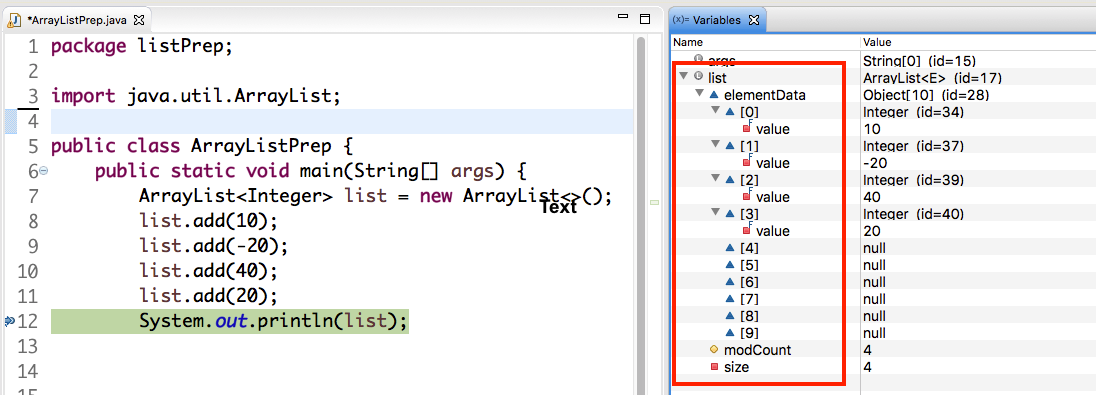
\includegraphics[scale=0.4]{images/elementData}
\end{figure}

\section{Custom Implementation of the essence of ArrayList class}

\subsection{Instance variables required}

The essential component of ArrayList class is that it should hold the items in an array, that \emph{grows} as and when required.

The maximum number of items that can be stored in the array is given by \texttt{data.length}.

But we also need to store how many items have been added so far.

So our instance variables are:

\begin{lstlisting}
class MyArrayList {
	private int[] data;
	private int nItems;	
}
\end{lstlisting}

\subsection{Adding items to the list}

Next, we need to have a method that adds an item to the list. For this, the core operation is,

\begin{lstlisting}
data[nItems] = itemToAdd;
nItems++;	
\end{lstlisting}

But what if the array is full? That is, items added so far equals the size of the array. Better to have that in a method of its own.

\subsubsection{Checking if array is full}

\begin{lstlisting}
public boolean isFull() {
	if(nItems == data.length)
		return true;
	else
		return false;
}
\end{lstlisting}

If the array is full, we need to grow it. Growing an array is a 3-step process.

\subsubsection{Growing the array}

Step 1: Create a bigger temporary array
\begin{lstlisting}
int[] temp = new int[data.length + 10];
\end{lstlisting}
Step 2: Copy over all items from your array to temporary array	
\begin{lstlisting}
for(int i=0; i < data.length; i++) {
	temp[i] = data[i];
}
\end{lstlisting}
Step 3: Copy reference held by temporary array into your array
\begin{lstlisting}
data = temp;
\end{lstlisting}

Putting this into one method,

\begin{lstlisting}
public void grow() {
	int[] temp = new int[data.length + 10]; //create bigger array
	
	for(int i=0; i < data.length; i++) { //copy items over 
		temp[i] = data[i];
	}
	
	data = temp; //re-reference instance variable array
}	
\end{lstlisting}

In our \texttt{add} method, we can check if array is full, and if it is, we grow it and proceed as normal.

\begin{lstlisting}
public void add(int item) {
	if(isFull())
		grow();
	//now not full anymore :)
	data[nItems] = item;
	nItems++;
}
\end{lstlisting}

\subsection{Removing an item}

While removing an item, you have a choice, to re-size the array to a smaller array or not. This is purely subjective and depends on what's more important - Time or Space? If time, then don't waste time in shrinking the array), and if space, then shrink the array. In our example, we don't (shrink the array).

We also have to move all subsequent items one space towards the beginning of the array.

\begin{lstlisting}
public Integer remove(int index) {
	if(index < 0 || index >= nItems) {
		return null; //advantage of return type being class
	}
	else {
		int result = data[index];
		for(int i=index; i < nItems - 1; i++) {
			data[i] = data[i+1];
		}
		nItems--;
		return result;
	}
}
\end{lstlisting}

As the last step, we will add two more methods. 

\begin{enumerate}
\item One that adds an item at a specific index. Just like remove, all subsequent items need to be moved towards the back (end) of the array by one index.

\begin{lstlisting}
public boolean add(int index, int item) {
	if(index < 0 || index > nItems)
		return false; //failure
	if(isFull())
		grow();
	for(int i=nItems; i > index; i--) {
		data[i] = data[i-1];
	}
	data[index] = item;
	return true;
}
\end{lstlisting}

\newpage

\item Good old toString!
\begin{lstlisting}
public String toString() {
	if(nItems == 0)
		return "[]";
	String result = "[";
	for(int i=0; i < nItems; i++) {
		result = result + data[i] + ", ";
	}
	int n = result.length();
	result = result.substring(0, n-2); //remove the last ", "
	result = result + "]";
	return result;
}
\end{lstlisting}
\end{enumerate}

\vskip 0.5cm

Putting it all together (and compacting a little bit), 

\vskip 0.5cm

\begin{lstlisting}[escapechar=^]
class MyArrayList {
	private int[] data;
	private int nItems;
	
	public Integer get(int index) {
		if(index < 0 || index >= nItems)
			return null;
		return data[index];
	}
	
	public boolean isFull() {
		return (nItems == data.length);  
		//returns outcome of expression
	}
	
	
	//continued on next page
	^\newpage^
	
	public void grow() {
		int[] temp = new int[data.length + 10];		
		for(int i=0; i < data.length; i++) {
			temp[i] = data[i];
		}
		data = temp;
	}		
	
	public void add(int item) {
		if(isFull())
			grow();
		data[nItems] = item;
		nItems++;
	}
	
	public Integer remove(int index) {
		if(index < 0 || index >= nItems)
			return null; 
		int result = data[index];
		for(int i=index; i < nItems - 1; i++)
			data[i] = data[i+1];
		nItems--;
		return result;
	}
}
\end{lstlisting}

\newpage

\subsection{Time complexity analysis}

\subsubsection{Accessing an item}

We need to understand how an array is stored to understand how array items are accessed.

An array is stored as a contiguous block of memory. 

As an example, if there is an array of 6 integers, 24 bytes are reserved (4 per integer). The first item is stored in the first four bytes, the second item in the next four bytes and so on.

<img src="./../fig/classesObjects/classesObjects-ClassUMLDiagram.png" alt="Drawing" width = "400"/>

Thus,
\begin{itemize}
  \item The address of the first item (at index 0) is the base address of the array (in this example, 600).
  \item The address of the second item (at index 1) is the base address of the array + 4 bytes.
  \item The address of the third item (at index 2) is the base address of the array + 2 * 4 bytes.
  \item $\cdots$  
  \item The address of the last item (at index 5) is the base address of the array + 5 * 4 bytes.
\end{itemize}

With a little tweak we can see:

\begin{itemize}
  \item Address(arr[\texttt{0}]) = baseAddress + \texttt{0} * 4
  \item Address(arr[\texttt{1}]) = baseAddress + \texttt{1} * 4
  \item Address(arr[\texttt{2}]) = baseAddress + \texttt{2} * 4
  \item $\cdots$  
  \item Address(arr[\texttt{arr.length - 1}]) = baseAddress + (\texttt{arr.length - 1}) * 4
\end{itemize}

Putting it all together,

\begin{verbatim}
(address of item at index idx) = (base address of array) + 
                                 (size of each item) * (idx);
\end{verbatim}

\subsubsection{Example: Accessing an item}

Let's say we want to access \texttt{arr[3]} in the following statement:

\begin{lstlisting}
int item = arr[3];
\end{lstlisting}

We start off with the reference held by \texttt{arr} and getting the base address (600). To that we add 3*4 = 12 (3 being the index and 4 being size of each item), giving us the starting address of the item 612. We grab 4 bytes starting at that address (so bytes 612 to 615) and present it packed as an integer: 90.

\begin{exercise}
Show the steps involved in accessing item \texttt{data[5]}.

\vskip 0.5cm
\begin{lstlisting}
double[] data = 	{12.5, 6.4, 8.5, 9.6, -3.4, -6.8, 0, -4.5};
\end{lstlisting}

<img src="./../fig/classesObjects/classesObjects-ClassUMLDiagram.png" alt="Drawing" width = "400"/>
\newline
\end{exercise}
\begin{answer}
address of \texttt{data[5]} = base address of \texttt{data} + 5 * 8\\
= 320 + 40 \\
= 360\\

\texttt{data[5]} = contents of memory from 360 to 367 \\
= -6.8	
\end{answer}

To access an item at index \texttt{idx}, we just have to perform one set of operation, and grab $x$ bytes from there (where $x$ is the size of each item of the array). 

The cost of this operation is fixed, irrespective of how big, or small, \texttt{idx} is. So, accessing an item in an ArrayList is $\mathcal{O}(1)$ operation in both best and worst cases.

\subsubsection{Inserting an item at a given index}

There are four cases for inserting an item:

\begin{enumerate}

\item Array is not full and you are inserting an item at the end of the array: None of items need to be moved, array doesn't need to be grown. $\mathcal{O}(1)$
\item Array is full and you are inserting an item at the end of the array: None of items need to be moved but array needs to be grown. Growing the array is $\mathcal{O}(n)$. Therefore, time complexity in this case is $\mathcal{O}(n)$.
\item Array is not full but you are inserting an item somewhere (not at the end): Some items need to be moved but array doesn't need to be grown. The worst case is when you are adding an item at index 0, in which case all items need to move, which is $\mathcal{O}(n)$. Therefore, time complexity in this case is also $\mathcal{O}(n)$.

For example, if there are 5 items currently being used in an array of size 8, and we try to insert an item 5.6 at index 0, all 5 items need to be moved forward.

<img src="./../fig/classesObjects/classesObjects-ClassUMLDiagram.png" alt="Drawing" width = "400"/>

\tikzstyle{occupied} = [draw,fill=red!10!white,minimum size=2.4em]
\tikzstyle{newItem} = [draw,fill=blue!20!white,minimum size=2.8em]
\tikzstyle{unoccupied} = [draw,fill=green!10!white,minimum size=2.4em]

\newcommand{\data}{{{12.5, 6.4, 8.5, 9.6, -3.4, 0, 0, 0},
					{12.5, 6.4, 8.5, 9.6, -3.4, -3.4, 0, 0},
					{12.5, 6.4, 8.5, 9.6, 9.6, -3.4, 0, 0},
					{12.5, 6.4, 8.5, 8.5, 9.6, -3.4, 0, 0},
					{12.5, 6.4, 6.4, 8.5, 9.6, -3.4, 0, 0},
					{12.5, 12.5, 6.4, 8.5, 9.6, -3.4, 0, 0},
					{6.4, 12.5, 6.4, 8.5, 9.6, -3.4, 0, 0}}}
					
\tikzstyle{line}=[draw] % here

<img src="./../fig/classesObjects/classesObjects-ClassUMLDiagram.png" alt="Drawing" width = "400"/>

\item Array is full and you are inserting an item somewhere (not at the end): Double whammy, but  $\mathcal{O}(n) + \mathcal{O}(n)$ is still $\mathcal{O}(n)$.
\end{enumerate}

\subsubsection{Removing an item at a given index}

There are two relevant cases for removing an item:

\begin{enumerate}
\item Removing the last item: No items need to be moved. $\mathcal{O}(1)$.
\item Removing the first item: All the items need to be moved. $\mathcal{O}(n)$.

For example, if there are 5 items currently being used in an array of size 8, and we try to remove the first item, all 5 items need to be moved backward by one.

<img src="./../fig/classesObjects/classesObjects-ClassUMLDiagram.png" alt="Drawing" width = "400"/>
\end{enumerate}

\tikzstyle{occupied} = [draw,fill=red!10!white,minimum size=2.4em]
\tikzstyle{unoccupied} = [draw,fill=green!10!white,minimum size=2.4em]

\newcommand{\data}{{{12.5, 6.4, 8.5, 9.6, -3.4, 0, 0, 0},
					{6.4, 6.4, 8.5, 9.6, -3.4, 0, 0, 0},
					{6.4, 8.5, 8.5, 9.6, -3.4, 0, 0, 0},
					{6.4, 8.5, 9.6, 9.6, -3.4, 0, 0, 0},
					{6.4, 8.5, 9.6, -3.4, -3.4, 0, 0, 0},
					{6.4, 8.5, 9.6, -3.4, -3.4, 0, 0, 0}}}
<img src="./../fig/classesObjects/classesObjects-ClassUMLDiagram.png" alt="Drawing" width = "400"/>

\vskip 1cm

Following table summarizes the time complexities of the various operations in an ArrayList:

\Large
\begin{center}
  \begin{tabular}{c|c|c}
    Operation & Best case & Worst case\\
    \hline
    Accessing an item & \color{ForestGreen} $\mathcal{O}(1)$ \color{black} & \color{ForestGreen} $\mathcal{O}(1)$ \color{black}\\
    \hline
    Inserting an item & \color{ForestGreen} $\mathcal{O}(1)$ \color{black} & \color{red} $\mathcal{O}(n)$ \color{black} \\
    \hline
    Removing an item & \color{ForestGreen} $\mathcal{O}(1)$ \color{black} & \color{red} $\mathcal{O}(n)$ \color{black}
  \end{tabular}
\end{center}
\normalsize

\section{Iterators}

Think of a bookmark that is placed between two pages such that the reader knows which page to read next.

An iterator offers the exact same functionality. 

\begin{enumerate}
  \item check if there is any item left after the current position of the iterator, and if so, access it. 
  \item check if there is any item before the current iterator position and again, if so, access it. 
  \item remove the next item (if any).
  \item change the value of the next item (if any).
  \item insert an item after the current iterator position.
\end{enumerate}

\vskip 1mm

Consider a list containing items 10, 70, 20, 90, 30, 80
\vskip 1mm

<img src="./../fig/classesObjects/classesObjects-ClassUMLDiagram.png" alt="Drawing" width = "400"/>

\newpage

Initial state of the iterator:
\vskip 1mm

<img src="./../fig/classesObjects/classesObjects-ClassUMLDiagram.png" alt="Drawing" width = "400"/>

\vskip 1mm

After accessing the first item (10):
\vskip 1mm

<img src="./../fig/classesObjects/classesObjects-ClassUMLDiagram.png" alt="Drawing" width = "400"/>

\vskip 1mm

After accessing the second item (70):
\vskip 1mm

<img src="./../fig/classesObjects/classesObjects-ClassUMLDiagram.png" alt="Drawing" width = "400"/>

\vskip 1mm

After accessing the third item (20):
\vskip 1mm

<img src="./../fig/classesObjects/classesObjects-ClassUMLDiagram.png" alt="Drawing" width = "400"/>

\vskip 1mm

After accessing the fourth item (90):
\vskip 1mm

<img src="./../fig/classesObjects/classesObjects-ClassUMLDiagram.png" alt="Drawing" width = "400"/>

\vskip 1mm

After accessing the fifth item (30):
\vskip 1mm

<img src="./../fig/classesObjects/classesObjects-ClassUMLDiagram.png" alt="Drawing" width = "400"/>

\vskip 1mm
				
After accessing the last item (80):
\vskip 1mm

<img src="./../fig/classesObjects/classesObjects-ClassUMLDiagram.png" alt="Drawing" width = "400"/>

\newpage

\subsection{Iterator implementation}

An iterator is created for a collection and since we are dealing with lists, we'll be creating a \texttt{ListIterator} as:

\begin{lstlisting}
Integer[] arr = {10,70,20,90,30,80};
ArrayList<Integer> list = new ArrayList(Arrays.asList(arr));

ListIterator<Integer> iter = list.listIterator();
\end{lstlisting}

You can check if there is an item "in front" of the iterator using \texttt{iter.hasNext()} which returns \texttt{true} if an items exists, \texttt{false} otherwise.

If an item exists, we can access it using \texttt{iter.next()}.

Thus, the traversal loop becomes,

\begin{lstlisting}
while(iter.hasNext()) {
	System.out.print(iter.next()+" ");
}
System.out.println();
\end{lstlisting}

You can also specify an index to the iterator from where it should begin.

\begin{lstlisting}
Integer[] arr = {10,70,20,90,30,80};
ArrayList<Integer> list = new ArrayList(Arrays.asList(arr));
ListIterator<Integer> iter = list.listIterator(3); 
//iterator is before item at index 3 (90)
\end{lstlisting}

Just like \texttt{hasNext(), next()}, you also have \texttt{hasPrevious(), previous()}.

In the example below, we start from the end of the list, iterating backwards.

\begin{lstlisting}
Integer[] arr = {10,70,20,90,30,80};
ArrayList<Integer> list = new ArrayList(Arrays.asList(arr));

//start from the end
ListIterator<Integer> iter = list.listIterator(list.size());
while(iter.hasPrevious()) { //any item BEFORE the iterator?
	System.out.print(iter.previous()+" ");
}
System.out.println();
\end{lstlisting}

Iterators can be passed to methods like any other object.
The following method removes all even items from the list for which the iterator is created.

\begin{lstlisting}
public static void removeEvens(ListIterator<Integer> iter) {
	while(iter.hasNext()) {
		if(iter.next() % 2 == 0) {
			//we have moved forward
			iter.previous(); //so, go back one space
			iter.remove(); 
		}
	}
}
\end{lstlisting}

You can add an item before the item following the iterator using \texttt{add(Object)}. The iterator remains at the same item as before and not before the newly added item.

The following method adds a zero in front of all items in the list for which the iterator is created. 

If the list was originally [10, 70, 20, 90], it would become [0, 10, 0, 70, 0, 20, 0, 90].

\begin{lstlisting}
public static void padZeroes(ListIterator<Integer> iter) {
	while(iter.hasNext()) {
		iter.add(new Integer(0)); 
		iter.next();
	}
}
\end{lstlisting}

\input{comp125lectureFooter}
